\documentclass[main.tex]{subfiles}

\begin{document}
\section{Modelli di classificazione}
I modelli che sono stati utilizzati per classificare sono l'analisi discriminante lineare e quadratica, il modello multinomiale e l'albero di classificazione.

Nella seguente tabella vengono riportate le percentuali di accuratezza raggiunte dalla classificazione effettuata da ogni modello nell'insieme di convalida.
\begin{table}[H]
\centering
\caption{Accuratezza per i modelli adattati.}
\begin{tabular}{cc}
\toprule
       Modello &  Accuratezza \% \\
\midrule
 Multinomiale &          85.87 \\
           QDA &          85.87 \\
 Decision Tree &          82.94 \\
           LDA &          72.66 \\
\bottomrule
\end{tabular}
\label{tab:acc}
\end{table}

La classificazione migliore è ottenuta con il modello multinomiale. L'importanza delle variabili esplicative è riassunta nella Figura~\ref{fig:importance-Tree}.
\begin{figure}[H]
	\centering
	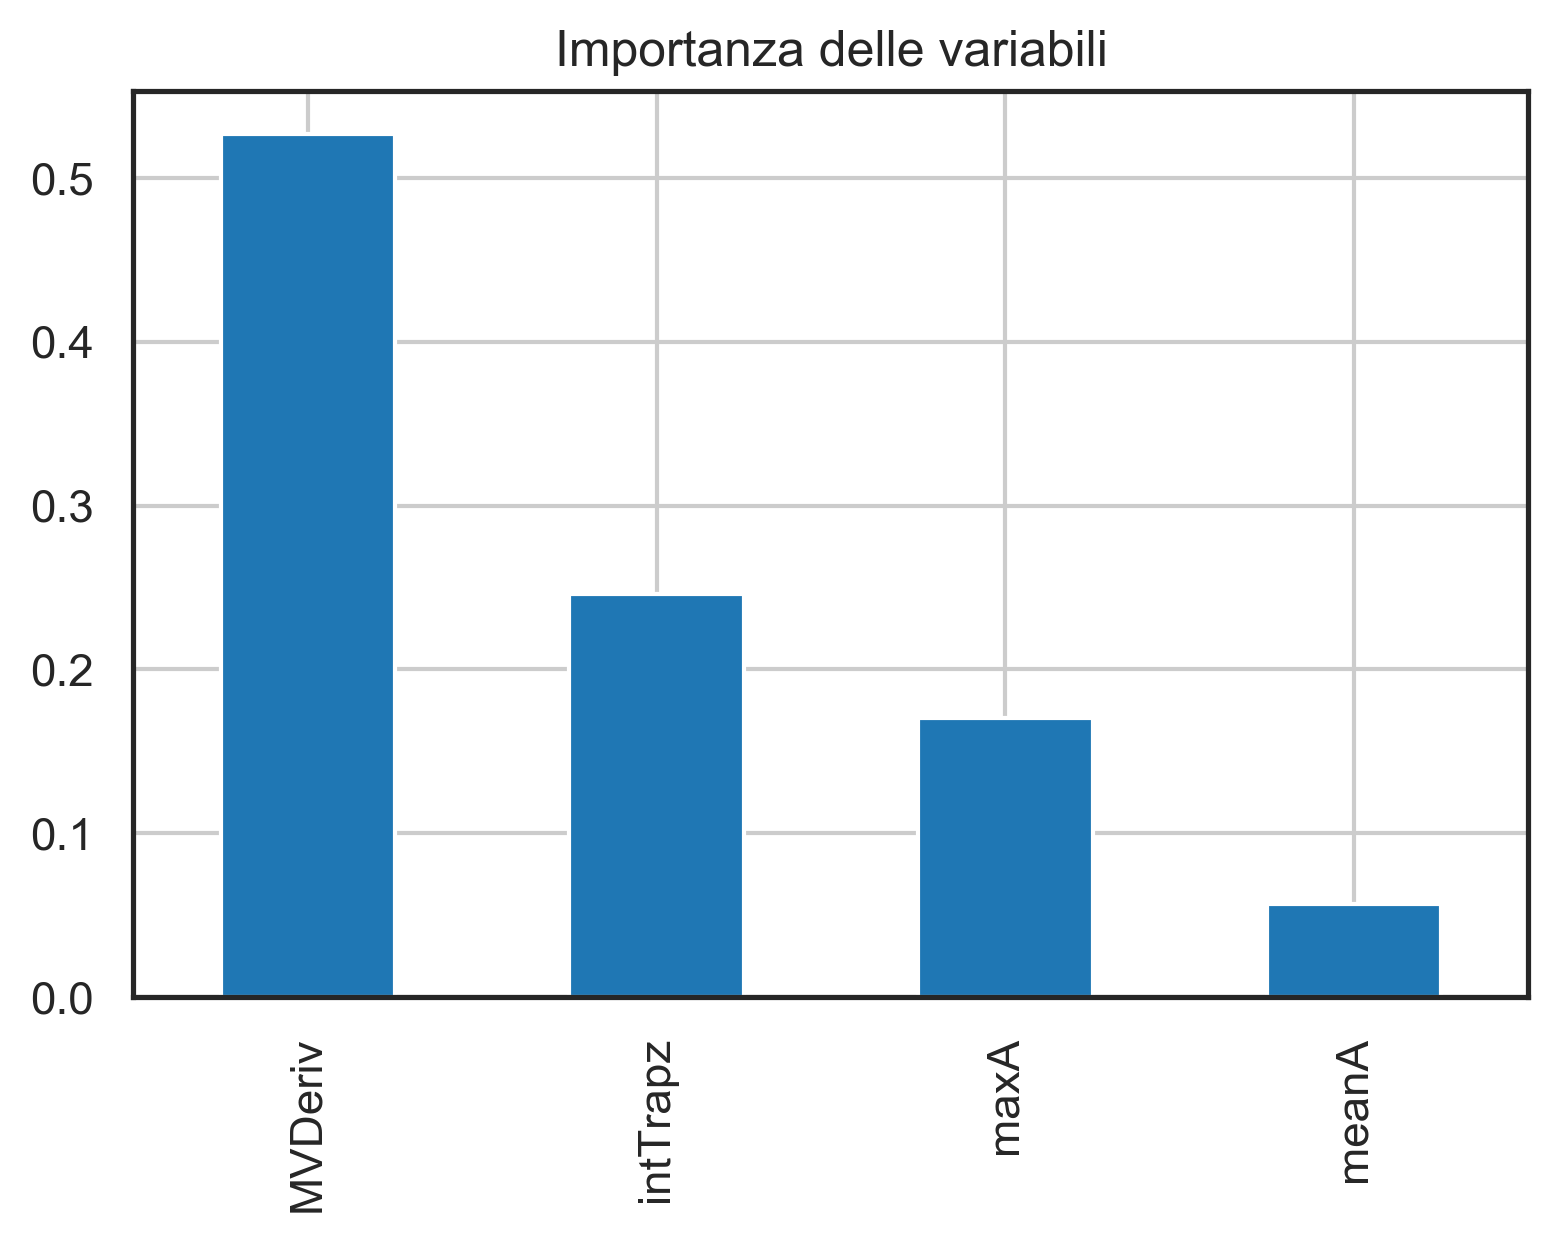
\includegraphics[width=.5\textwidth]{../../figure/importance-Tree.png}
	\caption{Importanza delle variabili ottenuta con l'albero di classificazione.}
	\label{fig:importance-Tree}
\end{figure}
Tale risultato è stato ottenuto dall'analisi condotta con l'albero di classificazione.

La matrice di confusione per il modello migliore è la seguente.
\begin{figure}[H]
	\centering
	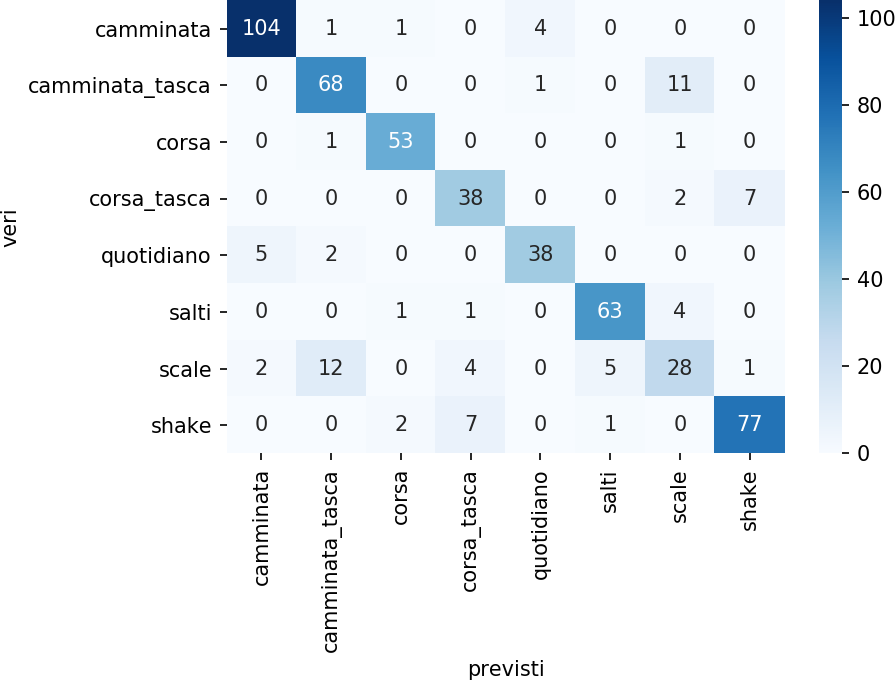
\includegraphics[width=.5\textwidth]{../../figure/confusionMatrix-Mn.png}
	\caption{Matrice di confusione ottenuta con il modello multinomiale.}
	\label{fig:mn}
\end{figure}
\end{document}